% This file is iccc.tex.  It contains the formatting instructions for and acts as a template for submissions to ICCC.  It borrows liberally from the AAAI and IJCAI formats and instructions.  It uses the files iccc.sty, iccc.bst and iccc.bib, the first two of which also borrow liberally from the same sources.


\documentclass[letterpaper]{article}
\usepackage{iccc}

\usepackage{graphicx}
\graphicspath{ {./images/}{./images} }
\usepackage{times}
\usepackage{helvet}
\usepackage{courier}
\pdfinfo{
/Title (Anything2vec: generalizing word2vec via the use of meaningful contexts)
/Subject (Proceedings of ICCC)
/Author (ICCC)}
% The file iccc.sty is the style file for ICCC proceedings.
%

\title{Anything2vec: generalizing word2vec via the use of meaningful contexts}
%\author{Dan Ventura\\
%Computer Science Department\\
%Brigham Young University\\
%Provo, UT 84602  USA\\
%ventura@cs.byu.edu\\
%}
\setcounter{secnumdepth}{0}

\begin{document} 
\maketitle
\begin{abstract}
\begin{quote}
In this paper we present a generalized approach to extend the use of word2vec for non traditional NLP (Natural Language Processing). In order to exemplify the idea we use tvtropes dataset (trope names and film names only) to create a text corupus in order to give contextual information to any pice of data.
\end{quote}
\end{abstract}

\section{Introduction}

% Motivation: we need to have a representation that is
% * That includes the context of the trope
% * relatively compact
% * capable of doing arithmetic
% * uniform for tropes and movies.

Our goal with this paper is to find a knowledge representation and methodology that let us to apply Machine Learning technics to tropes and films from tvtropes.org that let us to discover hidden conections between the different elements of this website. That new representation and methodology will let us, for example, to discover wich set of tropes will be affordable to create a new block buster film or a new best seller book.   

Tv Tropes (tvtropes.org) is a collaborative website created in 2004 to share information about tips, narrative or cinematographic techniques used in creative works such as movies, tv series, advertaising, videogames, sports, comics or books. Tvtropes.org defines "tropes" as: "A trope is a storytelling device or convention, a shortcut for describing situations the storyteller can reasonably assume the audience will recognize." Articles to describe tropes are writed usually with a very expresive and non formal vocabulary. Each film, tv serie or other fiction element usually include a description and a list of asociated tropes. Tropes pages usually contains a description followed by a list of films or a narrative resource that uses this trope.   

A first approach to represent films and tropes relationship to apply Machine Learning technics will be to create a multidimensional vector for each film, where each component will have 1 if the trope is included in this film or 0 if the trope is not included.  

   \{t1, t2, t3, ...., tn \}    
   
This approach have many disadvanteges. First of then are the difficult to deal with vectors with thousands dimensions. Other disavantage is that we have no possibility to do terms arithmetics. For example, will be interesting to Film1 - Western + Japanese = Film2 . The result of this arithmetic operation will be a film similar to Film1, but changing western style to japanese look. We can do this type of operations applying technics like word2vec \cite{mikolov2013}.  

Word2vec and similar technics are capable to add the context to the numerical vector that represents a word. This vector are created using the sorrounding terms included in a natural language text. In this way, the associated vector contains the meaning of this word extracted from the text used to build the model. After training process it is possible for example to ask Doctor - Man + Woman = ? . Logic tell us that the result will be Doctor (woman), instead, and it depends on how the text used to train the model "talk" about concepts, the result will be "nurse".  
   
After apply word2vect to a text corpus, a set of embeedings vectors will be created. The embeeding vector have information about the context of a certain word and it is easy to find the relationships with other terms in corpus. The challenge now is how to create a corpus that will be usefull to find relationships between tropes and films. Each film have a description and a list of tropes, and each trope have a description and a list of films that uses this trope. Initially our dataset obtained from tvtropes.org 13th december 2019 included 12360 films and 26742 different tropes (25405 after remove duplicates). The film with higher number of tropes has 1028 tropes and the film with minimum number of tropes has 0 tropes. 673258 pairs film-trope. 73917 duplicate values in pairs. 


\begin{figure}
	\centering
	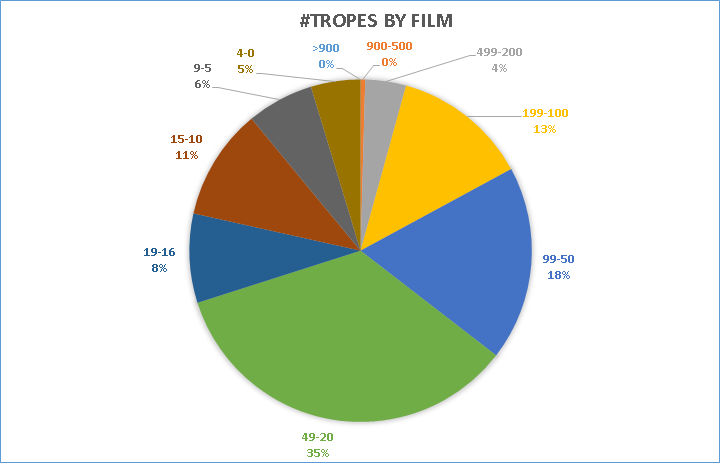
\includegraphics{images/num_tropes_by_film}
	\caption[Film distribution by num tropes]{Film distribution by num tropes}
	\label{fig:numtropesbyfilm}
\end{figure}










   

% How we want to solve that problem: we think that an adaptation of word2vec should be possible



% One of the most important elements in NLP (Natural Language Processing) is the context where words appear inside a text. One of the most popular algorithms to associte numerical vectors to words is word2vec \cite{mikolov2013}. This algorithm use words that are before and after a target word in order to contextualize words. But, what happend if we don't have a text to start analyzing words? What happend if we only have relationships between terms like this trope appear in this film? For this type of problem we purpouse a generalization in the use of word2vec algorithm that let to build a context for related terms. 

% (Talk about A Neural Network System for Transformation of Regional Cuisine Style \cite{kazama2018} and other non-NLP word2vec use like E-commerce in Your Inbox: Product Recommendations at Scale \cite{Grbovic2015} or Meta-Prod2Vec - Product Embeddings Using Side-Information for Recommendation \cite{vasile2016}

% How we do it:
% * Methodology for creating the context of every trope
% * Methdology for representing movies using trope vector
% * How we evaluate the goodness of the set of movies/tropes chosen.

% Our results
% * Clustering
% * Graph representation
% * Movie representation
% * Example of synthetic movie generation.

More information here about non-NLP word2vec
https://towardsdatascience.com/embeddings-with-word2vec-in-non-nlp-contexts-details-e879b093d34d
% Continue here

\section{State of the art}

\section{Methodology}

1. Download TvTropes dataset \\
2. Select films with number of tropes less than a certain number of tropes. The idea is to create a corpus with sentences constructed by permutations of sub-sets of tropes. \\
3. Build the corpus with permutations of tropes in each film \\
4. Build word2vec model. After that we will have a numerical vector for each trope. \\
5. Visualize tropes vector space in order to detect clusters and possible data organization. \\ 
6. Create a Vector for each film as the sumatory of all tropes vectors. \\

 


\section{Acknowledgments}


\bibliographystyle{iccc}
\bibliography{iccc}


\end{document}
